\documentclass[aspectratio=169]{beamer}
\usepackage[utf8]{inputenc}
\usepackage[T5]{fontenc}
\usepackage[vietnamese]{babel}
\usepackage{graphicx}
\usepackage{hyperref}
\usepackage{lmodern}

% Theme
\usetheme{Madrid}
\usecolortheme{whale}

% Metadata
\title[AI trong NN]{Ứng dụng AI trong Nông nghiệp}
\subtitle{Chương 3: Học máy (Machine Learning)}
\author{Giảng viên}
\institute{Đại học Đông Á}
\date{\today}

\begin{document}

\begin{frame}
    \titlepage
\end{frame}

\begin{frame}{Nội dung chính}
    \tableofcontents
\end{frame}

\section{Giới thiệu chung}
\begin{frame}{Học máy (Machine Learning) là gì?}
    \begin{itemize}
        \item Là một lĩnh vực của Trí tuệ Nhân tạo (AI) giúp máy tính học hỏi từ dữ liệu.
        \item Sử dụng các thuật toán liên tục học hỏi từ dữ liệu có sẵn dưới dạng dữ liệu huấn luyện (training data).
        \item \textbf{Mục tiêu:} Tạo ra mô hình có thể xấp xỉ dữ liệu chưa từng thấy và đưa ra kết quả, dự đoán hoặc quyết định chính xác.
        \item Khác với lập trình truyền thống: Không cần lập trình rõ ràng mọi quy tắc, máy tính tự rút ra quy luật.
    \end{itemize}
\end{frame}

\begin{frame}{Học lặp từ dữ liệu (Iterative Learning from Data)}
    \begin{itemize}
        \item Các mô hình học máy luôn được huấn luyện từ các bộ dữ liệu khác nhau trước khi được triển khai.
        \item \textbf{Mô hình trực tuyến (Online):} Liên tục nhận dữ liệu mới và thích ứng (học lặp).
        \item \textbf{Mô hình ngoại tuyến (Offline):} Được huấn luyện tĩnh, khi triển khai không thay đổi và luôn dựa vào kiến thức đã học.
        \item \textbf{Ứng dụng thực tế:} Phân tích dữ liệu lịch sử để dự đoán trong tương lai hoặc phân tích dữ liệu thực tế liên tục.
    \end{itemize}
\end{frame}

\begin{frame}{Mô hình Học máy}
    \begin{center}
        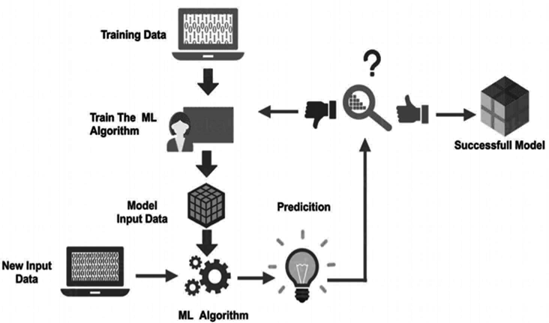
\includegraphics[height=0.7\textheight]{chap3_img_1_0.png}
        
        \textit{Hình 3.1: Mô hình Học máy cơ bản}
    \end{center}
\end{frame}

\section{Phương pháp tiếp cận Học máy}
\begin{frame}{Các phương pháp tiếp cận Học máy}
    Tùy vào loại bài toán, mục tiêu và dữ liệu, chúng ta sử dụng các kỹ thuật học máy khác nhau:
    \vspace{0.5cm}
    \begin{enumerate}
        \item \textbf{Học có giám sát (Supervised Learning)}
        \item \textbf{Học không giám sát (Unsupervised Learning)}
        \item \textbf{Học bán giám sát (Semi-supervised Learning)}
        \item \textbf{Học tăng cường (Reinforcement Learning)}
    \end{enumerate}
\end{frame}

\subsection{Học có giám sát}
\begin{frame}{1. Học có giám sát (Supervised Learning)}
    \begin{itemize}
        \item \textbf{Khái niệm:} Mô hình được cung cấp dữ liệu đã được gán nhãn (labeled data) để huấn luyện.
        \item Giống như có một người ``thầy'' hướng dẫn chỉ cho mô hình câu trả lời đúng.
        \item Tìm hàm ánh xạ (mapping function): $Y = f(X)$ sao cho từ đầu vào mới có thể dự đoán được đầu ra $Y$.
        \item \textbf{Chia thành 2 bài toán chính:}
        \begin{itemize}
            \item \textbf{Phân loại (Classification):} Đầu ra rời rạc (Ví dụ: Cây khỏe / Cây bệnh).
            \item \textbf{Hồi quy (Regression):} Đầu ra liên tục (Ví dụ: Năng suất vụ mùa tính bằng tấn, nhiệt độ).
        \end{itemize}
    \end{itemize}
\end{frame}

\begin{frame}{Phân loại (Classification)}
    \begin{itemize}
        \item Một vấn đề phân loại được đặt tên khi chúng ta có hiệu suất được phân loại (categorized) rõ ràng.
        \item \textbf{Ứng dụng trong nông nghiệp:}
        \begin{itemize}
            \item Dựa vào hình ảnh, phân loại đây là loại cây trồng nào.
            \item Nhận diện hạt giống có bị sâu bệnh hay không.
            \item Phân loại trái cây (Loại 1, Loại 2, \dots).
        \end{itemize}
        \item \textbf{Thuật toán tiêu biểu:} Cây quyết định (Decision Tree), Random Forest, KNN, Logistic Regression.
    \end{itemize}
\end{frame}

\begin{frame}{Hồi quy (Regression)}
    \begin{itemize}
        \item Một vấn đề hồi quy được đặt tên khi có giá trị đầu ra là số thực.
        \item \textbf{Ứng dụng trong nông nghiệp:}
        \begin{itemize}
            \item Dự đoán năng suất tính theo kilogram hoặc tấn trên mỗi hecta.
            \item Dự đoán giá bán nông sản trên thị trường theo các điều kiện kinh tế.
            \item Xác định lượng nước, phân bón tối ưu dựa trên độ ẩm và tính chất đất.
        \end{itemize}
        \item \textbf{Thuật toán tiêu biểu:} Hồi quy tuyến tính (Linear Regression), Support Vector Regression.
    \end{itemize}
\end{frame}

\subsection{Học không giám sát}
\begin{frame}{2. Học không giám sát (Unsupervised Learning)}
    \begin{itemize}
        \item \textbf{Khái niệm:} Mô hình huấn luyện trên dữ liệu \textbf{không được gán nhãn} (unlabeled data).
        \item Hoạt động độc lập mà không cần sự can thiệp của con người (không có câu trả lời đúng).
        \item Mô hình tự tìm các mẫu (patterns), phân cụm (clusters) hoặc cấu trúc ẩn bên trong dữ liệu.
        \item \textbf{Ứng dụng trong nông nghiệp:}
        \begin{itemize}
            \item Phân cụm các vùng đất canh tác có tính chất (độ pH, khoáng chất) tương đồng.
            \item Phân tích đặc tính thị trường hoặc hành vi mua hàng.
            \item Tiền xử lý dữ liệu để gắn nhãn tự động một phần.
        \end{itemize}
    \end{itemize}
\end{frame}

\begin{frame}{Các bài toán trong Học không giám sát}
    \begin{itemize}
        \item \textbf{Phân cụm (Clustering):} Gom nhóm dữ liệu thành các cụm có tính chất giống nhau. 
        \begin{itemize}
            \item Thuật toán: K-Means Clustering, Hierarchical Clustering.
        \end{itemize}
        \item \textbf{Luật kết hợp (Association Rules):} Tìm các quy tắc mô tả phần lớn dữ liệu.
        \begin{itemize}
            \item Ví dụ: Phát hiện những loại cây nào thường mắc bệnh chung với nhau trong một số điều kiện thời tiết nhất định.
        \end{itemize}
    \end{itemize}
\end{frame}

\subsection{Thuật toán phổ biến}
\begin{frame}{Các thuật toán Học máy tiêu biểu}
    \begin{itemize}
        \item \textbf{Decision Tree (Cây quyết định):} Tạo ra cấu trúc cây để ra quyết định dựa trên điều kiện của dữ liệu đầu vào.
        \item \textbf{Random Forest (Rừng ngẫu nhiên):} Tập hợp của nhiều cây quyết định nhằm tăng độ chính xác và giảm nhiễu.
        \item \textbf{K-Nearest Neighbors (KNN):} Phân loại đối tượng dựa vào số đông của K đối tượng hàng xóm gần nhất.
        \item \textbf{Support Vector Machines (SVM):} Vẽ ranh giới phân chia tốt nhất giữa các lớp dữ liệu.
    \end{itemize}
\end{frame}

\begin{frame}{Minh họa thuật toán: Cây quyết định}
    \begin{columns}
        \begin{column}{0.4\textwidth}
            \begin{itemize}
                \item \textbf{Cơ chế hoạt động:} Phân chia dữ liệu dựa trên các câu hỏi điều kiện (Yes/No) tại mỗi nút (node).
                \item \textbf{Cấu trúc:} Bao gồm nút gốc, các nút nhánh và nút lá (kết quả phân loại).
                \item Trực quan, dễ hiểu, mô phỏng cách con người ra quyết định.
            \end{itemize}
        \end{column}
        \begin{column}{0.6\textwidth}
            \begin{center}
                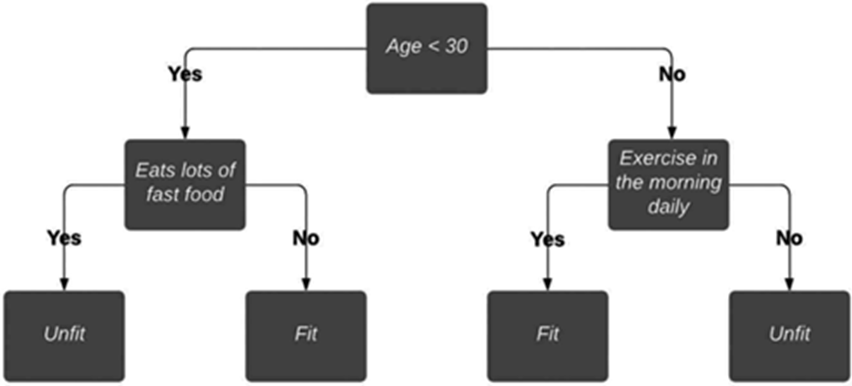
\includegraphics[width=\textwidth]{chap3_img_6_0.png}
                
                \vspace{0.2cm}
                \textit{Hình 3.2: Cây quyết định (Decision Tree)}
            \end{center}
        \end{column}
    \end{columns}
\end{frame}

\begin{frame}{Minh họa thuật toán: Máy véc-tơ hỗ trợ (SVM)}
    \begin{columns}
        \begin{column}{0.4\textwidth}
            \begin{itemize}
                \item \textbf{Cơ chế hoạt động:} Tìm ra một siêu phẳng (hyperplane) biên giới tối ưu nhất để phân tách các lớp dữ liệu.
                \item \textbf{Support Vectors:} Là các điểm dữ liệu nằm gần ranh giới phân chia nhất.
                \item Hiệu quả rất cao trong các bài toán phân loại phức tạp và không gian nhiều chiều.
            \end{itemize}
        \end{column}
        \begin{column}{0.6\textwidth}
            \begin{center}
                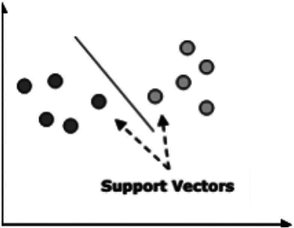
\includegraphics[width=\textwidth]{chap3_img_6_1.png}
                
                \vspace{0.2cm}
                \textit{Hình 3.3: Máy véc-tơ hỗ trợ (SVM)}
            \end{center}
        \end{column}
    \end{columns}
\end{frame}

\section{Kết luận}
\begin{frame}{Kết luận}
    \begin{itemize}
        \item Học máy là công cụ cốt lõi trong Trí tuệ Nhân tạo để phân tích dữ liệu hiệu quả.
        \item Nông nghiệp hưởng lợi rất lớn từ Học máy qua việc phân tích lượng dữ liệu khổng lồ từ cảm biến, camera và báo cáo mùa vụ.
        \item Việc lựa chọn thuật toán (Có giám sát, Không giám sát) phụ thuộc chặt chẽ vào loại dữ liệu thu thập được và mục tiêu giải quyết của người nông dân hoặc chuyên gia nông nghiệp.
    \end{itemize}
\end{frame}

\end{document}
